\section{Method}\label{sec:method}

The statedness diagnostic (\S\ref{sec:design}) measures the bias that SDA (\S\ref{sec:sda}) targets.

\subsection{Statedness Diagnostic}\label{sec:design}

\paragraph{Episodes.}
GPT-4.1 builds Decoupled episodes: passages about named people, useful concepts, future questions and answers. Answers are absent from passages and candidates; questions connect to passages only through the person's name. We evaluate 363 test and 316 held-out episodes, checked by rule-based filters and a blind alias filter (App.~\ref{app:benchmarks}). Training and validation use Explicit and Implied-answer constructions; separate development sets guide configuration (App.~\ref{app:fresh}; App.~\ref{app:training}).

\paragraph{Statedness conditions.}
Table~\ref{tab:design} crosses useful-concept and distractor statedness using Figure~\ref{fig:episode}. Conditions A--D measure $\mathrm{WR}_{0,1}$, $\mathrm{WR}_{0,0}$, $\mathrm{WR}_{1,1}$ and $\mathrm{WR}_{1,0}$ (Eq.~\eqref{eq:winrate}).
\begin{table*}[t]
\centering
\small
\caption{Four statedness conditions using Figure~\ref{fig:episode}. ``Named'' appends ``The passage also mentions mesopotamia.'' to the passage; usefulness is unchanged.}
\label{tab:design}
\renewcommand{\arraystretch}{1.1}
\begin{tabular}{@{}cllcll@{}}
\toprule
Condition & Useful concept & Distractor & Win rate & Example & Role \\
\midrule
\textbf{A} & Implied & Stated & $\mathrm{WR}_{0,1}$ & \texttt{mesopotamia} vs.\ \texttt{silt} & Exposes the Statedness Bias \\
\textbf{B} & Implied & Unstated & $\mathrm{WR}_{0,0}$ & \texttt{mesopotamia} vs.\ \texttt{levant} & Tests recognition \\
\textbf{C} & Stated & Stated & $\mathrm{WR}_{1,1}$ & named \texttt{mesopotamia} vs.\ \texttt{silt} & Finds useful passage words \\
\textbf{D} & Stated & Unstated & $\mathrm{WR}_{1,0}$ & named \texttt{mesopotamia} vs.\ \texttt{levant} & Sanity check \\
\bottomrule
\end{tabular}
\end{table*}


Condition A pairs an implied useful concept with a stated distractor, so usefulness and statedness favor different candidates; it tests whether passage words displace useful concepts. Condition B uses an unstated distractor instead, testing usefulness discrimination at fixed statedness. Because A and B share implied useful concepts, A below B identifies the Statedness Bias. Conditions C and D repeat both comparisons with a stated useful concept: C tests usefulness discrimination among passage words, and D, where usefulness and statedness agree, is a sanity check.

\paragraph{Candidate pools.}
The original pool contains 1,607 candidates, 4.43 per episode. In 95\% of episodes, the useful concept is the sole unstated candidate, making statedness a shortcut to usefulness.

The main statedness-balanced pool removes this shortcut. An LLM generates same-category distractors absent from and not implied by the passage, forming the pool with unstated distractors. In fixed test-set order, odd-position episodes keep their passage and add the first four unstated distractors from the pool with unstated distractors; even-position episodes append ``The passage also mentions \emph{useful concept}.'' and add the first three. All original candidates remain, added candidates are distractors, and questions, answers and original utility labels stay fixed.

The pool contains 190 stated and 173 implied episodes, with 7.93 candidates per episode. Useful concepts constitute 13.3\% of stated and 12.0\% of unstated candidates. Statedness alone ranks at chance: pooled AUC 0.515 and within-episode AUC 0.516. Controls test naming (useful-concept-named control, naming-balanced pool), candidate composition (pool with unstated distractors, enlarged pool) and passage dependence (paired-passage set, passage replacement; App.~\ref{app:pools}).

\subsection{Self-Distilled Admission}\label{sec:sda}

\begin{figure*}[t]
\centering
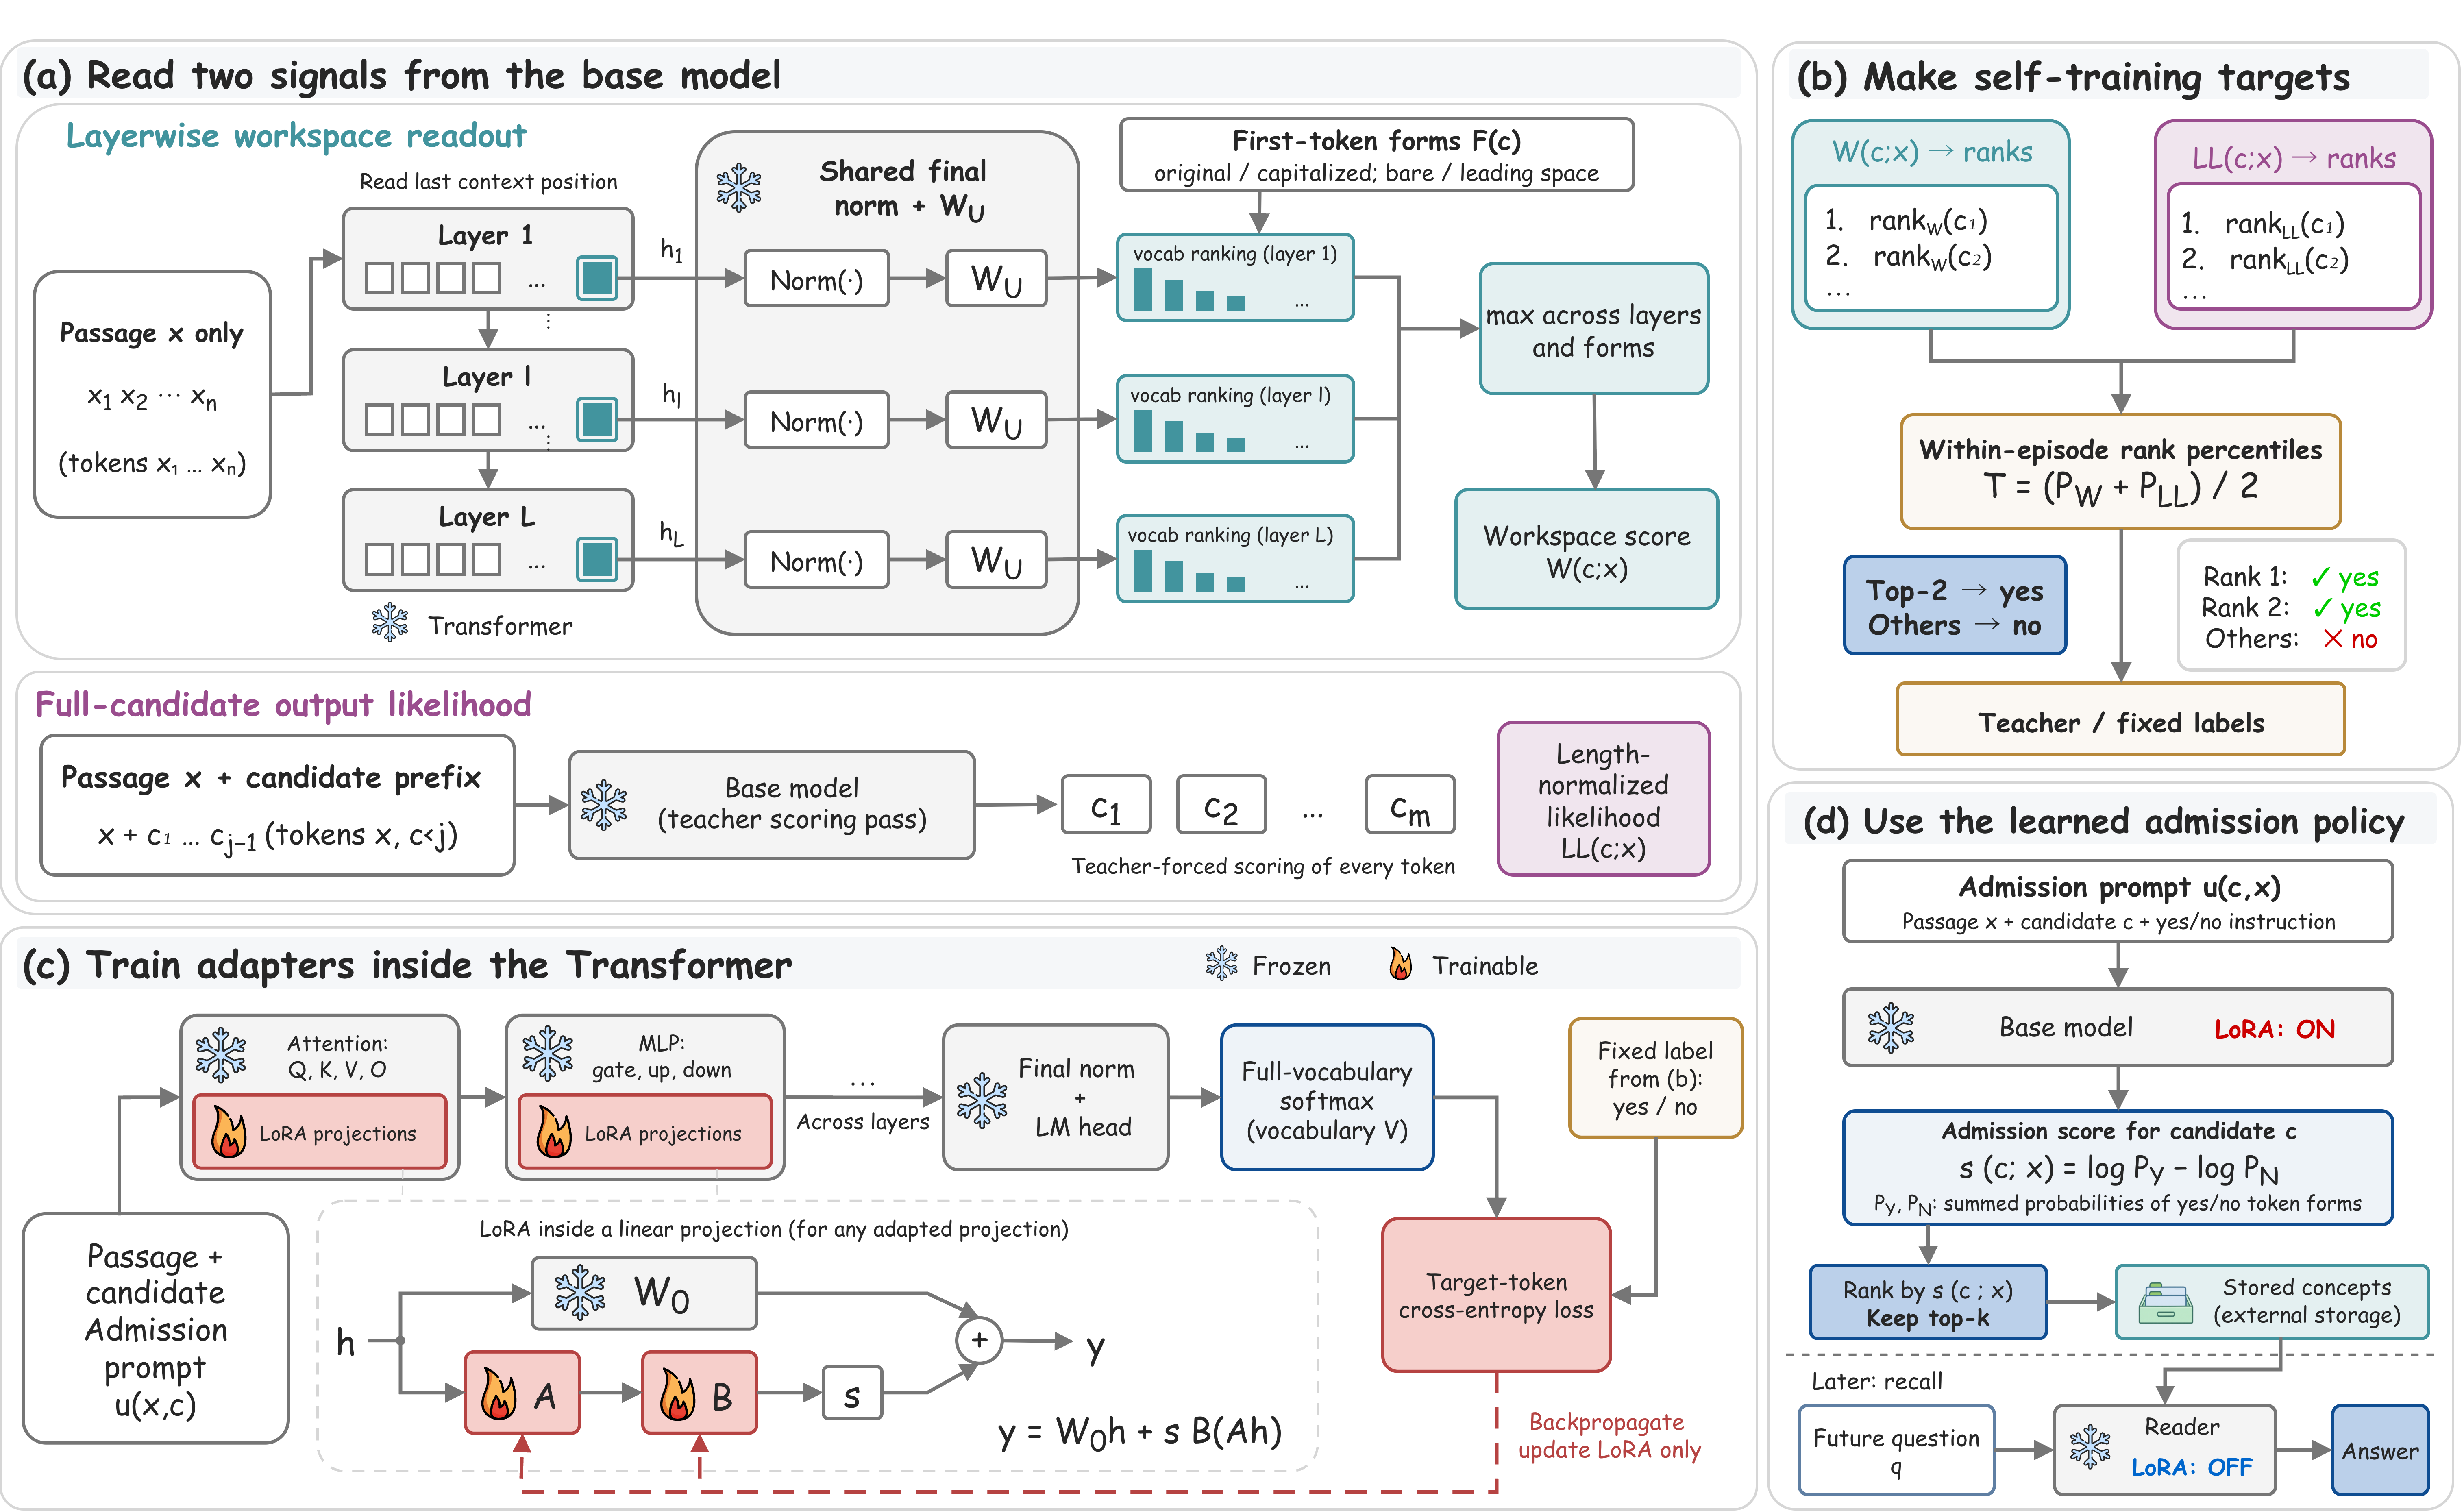
\includegraphics[width=0.9\textwidth]{figures/fig2.png}
\caption{(a) The logit-lens readout and output likelihood score candidates. (b) Averaged within-episode rank percentiles form $T(c;x)$: the top two receive \emph{yes}, the rest \emph{no}. (c) Target-token cross-entropy trains only the adapter through the importance prompt $u(c,x)$. (d) Admission alone uses the adapter and stores the top-$k$ candidates under $s_\theta(c;x)$; the frozen reader answers later with the adapter off.}
\label{fig:sda}
\end{figure*}

SDA trains the importance judgment because the model already recognizes implied useful concepts (Condition B, \S\ref{sec:bias}; internal signals, \S\ref{sec:knowledge}). A LoRA adapter learns labels from the model's own signals through the importance prompt and serves only admission (Figure~\ref{fig:sda}; Algorithm~\ref{alg:sda}, App.~\ref{app:training}).

\paragraph{Teacher signals.}
At the final passage position, the logit lens projects hidden states as $z_\ell(x)=W_U\,\mathrm{LN}(h_\ell(x))$ for $1\leq\ell\leq L$. Here $h_\ell$ is the residual state after layer $\ell$ for $\ell<L$; $h_L$ is the final state returned by the model. The readout takes the peak reciprocal rank:
\begin{equation}
\begin{split}
\mathrm{rank}_\ell(t)&=1+|\{v:z_{\ell,v}>z_{\ell,t}\}|,\\
R(c;x)&=\max_{\substack{1\leq\ell\leq L\\t\in F(c)}}\frac{1}{\mathrm{rank}_\ell(t)}.
\end{split}
\label{eq:wrr}
\end{equation}
$F(c)$ contains distinct first tokens of bare and leading-space forms of $c$, in original and capitalized case. One forward pass serves all candidates. Output likelihood is $\mathrm{LL}(c;x)=\log p(c\mid x)/|c|$, where $|c|$ is token length. Within-episode ranks place the signals on a common scale.

\paragraph{Labels and distillation.}
Let $P_R$ and $P_{\mathrm{LL}}$ be within-episode mid-rank percentiles, with ties assigned their mean rank. The teacher averages them:
\begin{equation}
T(c;x)=\tfrac12\bigl(P_R(c;x)+P_{\mathrm{LL}}(c;x)\bigr).
\label{eq:teacher}
\end{equation}
The top two candidates receive $\tilde y=1$ (\emph{yes}), the rest $\tilde y=0$ (\emph{no}); candidate order breaks ties.

With base weights frozen, rank-16 LoRA \citep{hu2021lora} on every attention and feed-forward projection minimizes target-token cross-entropy through the importance prompt:
\begin{equation}
\begin{split}
\mathcal L(\theta)={}&-\frac{1}{|\mathcal D|}\sum_{(x,c)\in\mathcal D}\\
&\quad\cdot\log p_\theta\!\left(\tau(\tilde y(c;x))\mid u(c,x)\right).
\end{split}
\label{eq:loss}
\end{equation}
$\mathcal D$ contains passage--candidate pairs; $\tau$ maps labels to target tokens. Probabilities are vocabulary-normalized; prompt tokens are masked. Training runs two epochs. We retain the earliest checkpoint with highest validation within-episode AUC; gold utility labels serve only validation (App.~\ref{app:training}). Results average three training runs.

\paragraph{Why the student can exceed its teacher.}
Condition B tests discrimination the judgment already possesses. Training retains the importance prompt while teacher labels counter its preference for passage words. The student thus starts with useful discrimination beyond its supervision, the premise of weak-to-strong generalization \citep{burns2023weak}; \S\ref{sec:learns} compares student and teacher.

\paragraph{Serving.}
SDA ranks by $s_\theta$ (Eq.~\eqref{eq:score}) and stores the top $k$, using one yes/no forward pass per candidate with passage prefix caching \citep{kwon2023pagedattention}; the reader answers with the adapter off (App.~\ref{app:timing}).
